\chapter{Results}\label{chap:results}
\thispagestyle{fancy}

\section{Cataclysmic Variables }
From the population of known CV candidates in NGC 6397 we were able to get the spectra of five of them (see fig.~\ref{fig:todosspectra}). In addition to recovering 3 of the previously detected cataclysmic variables, we have obtained the spectra for the first time of two CV candidates (U10 and U22 see figures \ref{fig:U10spectra} and \ref{fig:U22spectra}). Their spectra confirms that these star are CVs, as suggested by their X-ray data \citep{grindlay_chandra_2001}. With the exception of U10, all the obtained spectra lie within a distance of $11"$ from the cluster center. Their spectra is obtained from two observing night of the cluster center. The total exposure time is 340 seconds from a total of 8 different exposures ($4 \times 25$ s and $4 \times 60$ s). U10 lies at a distance of $1.21'$ and was also observed during two different nights. The total exposure time on U10 is 265 seconds divided in 9 different short exposures ($5 \times 25$ s and $4 \times 35$ s). 

\begin{figure}[h]
        \centering
        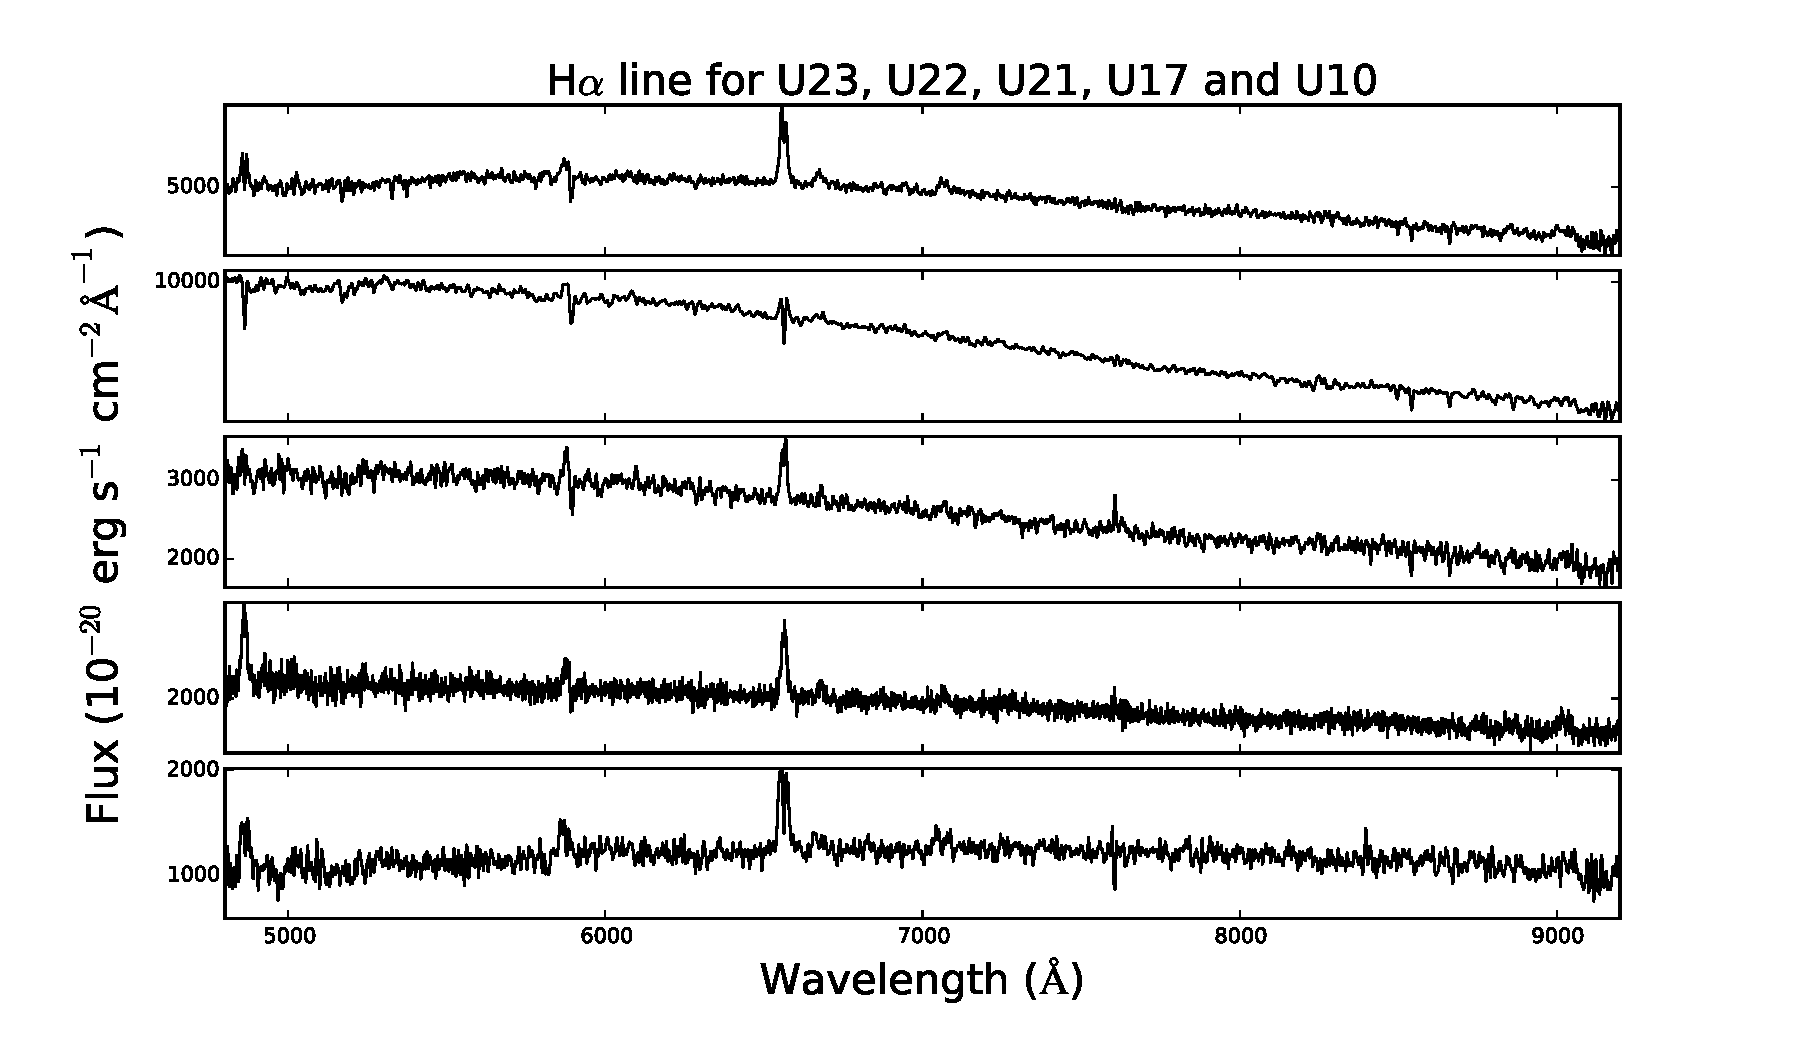
\includegraphics[scale=.6]{assets/images/todostodos.pdf}
\caption{Obtained spectra from CVs in NGC 6397. Three of them have been previously identified as CVs: U23, U21 and U17 \citep{grindlay_spectroscopic_1995,edmonds_cataclysmic_1999}. U22 and  U10 are CV candidates that have been first confirmed with spectroscopy. All CVs show strong Balmer lines ($6563 \text{ and } 4861 \mathring{ A}$). The IDs are from \citep{bogdanov_chandra_2010}.}
\label{fig:todosspectra}
\end{figure}

\begin{figure}[h]
        \centering
        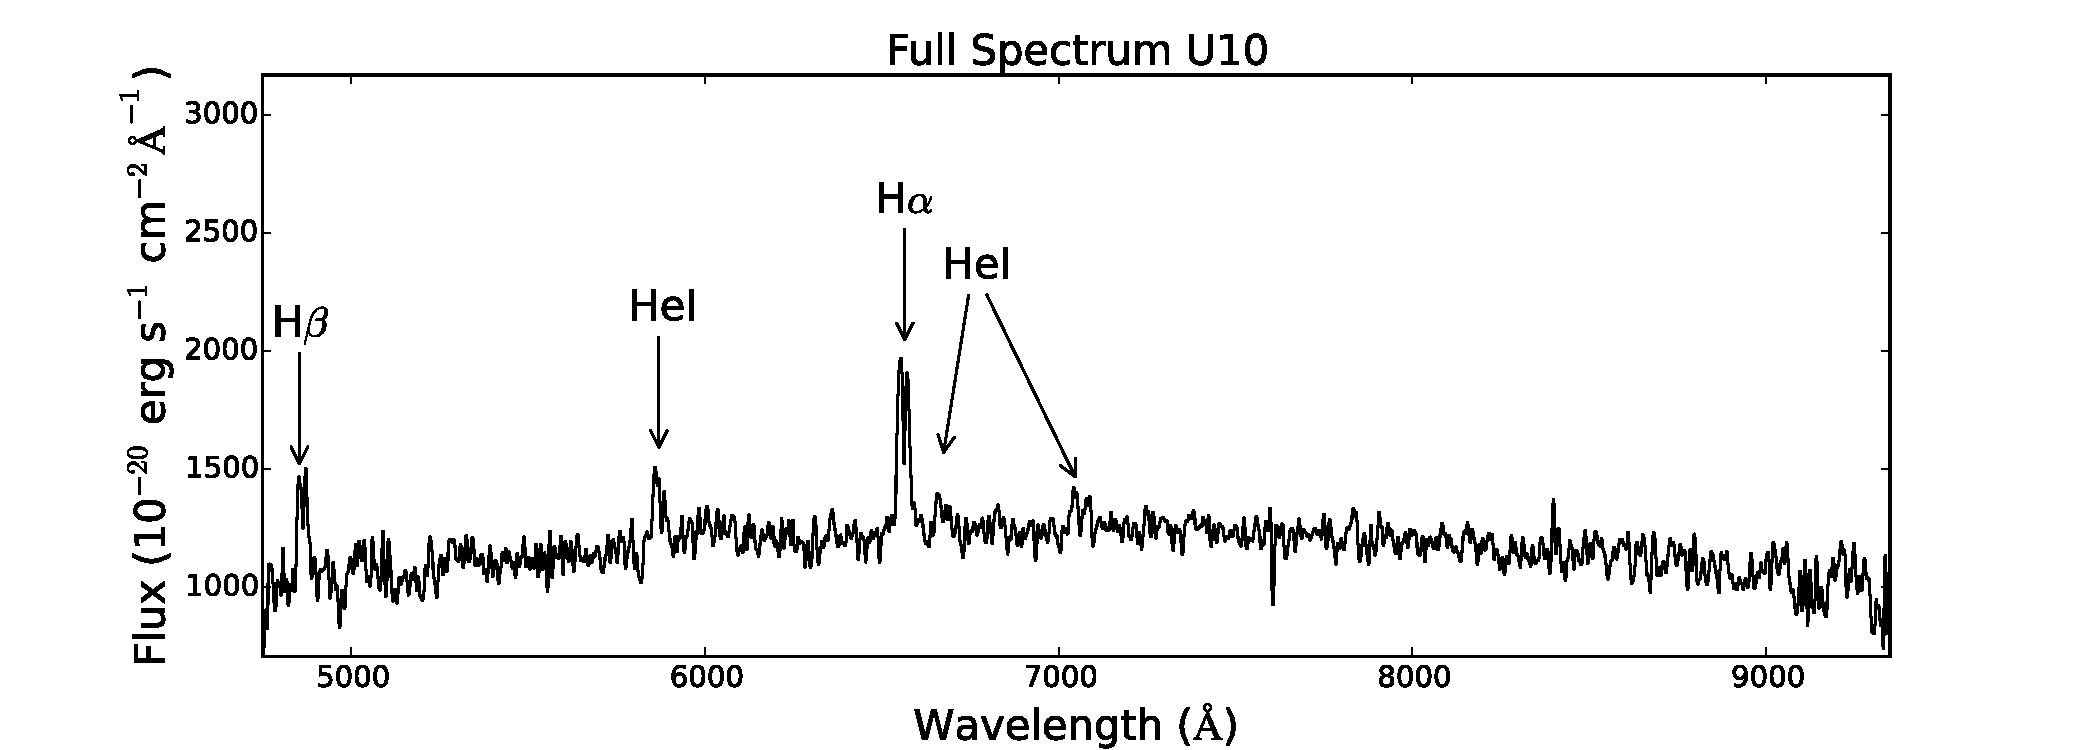
\includegraphics[scale=.5]{assets/images/U10full.pdf}
\caption{Spectrum of U23 with strong Hydrogen double peaked emission (characteristic of an accretion disk), and a strong Helium I lines. }
\label{fig:U10spectra}
\end{figure}

\begin{figure}[h!]
        \centering
        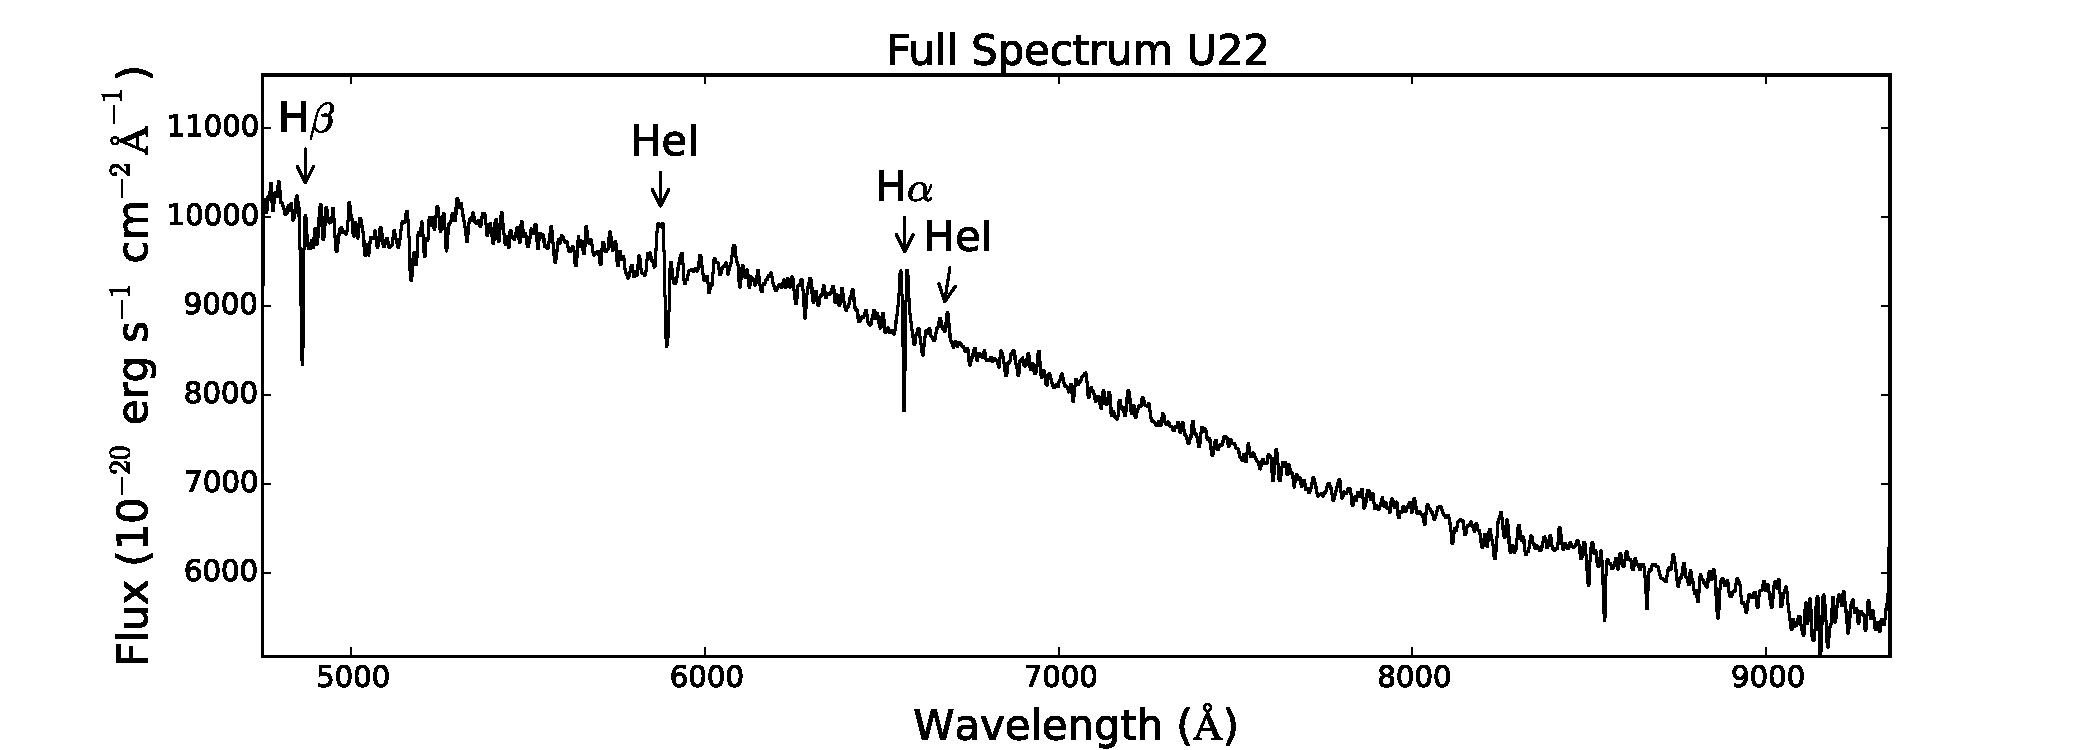
\includegraphics[scale=.5]{assets/images/U22full.pdf}
\caption{Spectrum of U22 with strong H$\alpha$ double peaked emission, absorption in the H$\beta$ line, and Helium I lines.}
\label{fig:U22spectra}
\end{figure}



\subsection{Variability}

From the extracted CV spectra we calculated the magnitudes in the R band (in the VEGA system), and compare it to the magnitude seen in 2010 by the Hubble space telescope as reported by \cite{cohn_identification_2010}. The results are summarized in table~\ref{tab:truthTables}. The CVs show moderate amplitude variability between the two observing times. This suggest that the majority of the CVs were observed during quiescence and not during an outburst. For some CVs like U22 where the change magnitude is bigger the possibility of being observed during outburst is not ruled out. A dwarf nova eruption can result in moderate magnitude changes of $\sim 2$. This have been observed for U17 and U19. They have been reported to undergo dwarf nova eruptions with amplitudes of 1.8 and 2.7 magnitudes \citep{shara_erupting_2005}. 

%Further analysis of the spectra is needed to rule out the outburst scenario.  

\begin{table}[h]
\centering
\begin{tabular}{|c|c|c|}
\hline
\textbf{CV} & \textbf{R Magnitude (2014)} & \textbf{R (Cohn et al. 2010)} \\ \hline
U17         & 20.12                       & 18.52                          \\ \hline
U23         & 19.15                       & 17.88                       \\ \hline
U10         & 20.7                        & 19.14                     \\ \hline
U21         & 19.79                       & 19.82                    \\ \hline
U22         & 18.54                       & 20.15                              \\ \hline

\end{tabular}
   \caption{Magnitudes in the R band for the 5 CVs detected by MUSE in 2014 and the R magnitudes in 2010 studied by \cite{cohn_identification_2010}. Some CVs show small magnitude variability between the two epochs ($\sim 1$ magnitude).}
    \label{tab:truthTables}   
\end{table}





\begin{comment}
Results:

    Spectra:
        “Brights”
        “Faint”
        ’Intermediate"
        Neutron Star
    Variability:
        Magnitude now, in (Cohn et al. 2010) and (Kaluzny et al. 2006) range
    Mass estimation:
        DP/FWHM vs. q according to [casares_mass_2016]
    Secondary Star:
        M star spectra from (Husser et al. 2016)
        Lack or presence
Neutron star. 

Form using the
\hline
\textbf{CV} & \textbf{R Magnitude (2014)} & \textbf{R (Cohn et al. 2010)} & EW H$\beta$ ($\mathring{A})$ \\ \hline
U17         & 20.12                       & 18.52                         & $11.65 \pm 0.17$             \\ \hline
U23         & 19.15                       & 17.88                         & $15.13 \pm 0.7$              \\ \hline
U10         & 20.7                        & 19.14                         & $15.44 \pm 0.2$              \\ \hline
U21         & 19.79                       & 19.82                         & -                            \\ \hline
U22         & 18.54                       & 20.15                         & -                            \\ \hline
\end{tabular}
\end{comment}

\subsection{Mass ratio}

As seen in figure~\ref{fig:todosspectra} a common feature in all of the extracted spectra is the presence of the Balmer lines. These are a set of spectral line emissions of the hydrogen atom. In the MUSE spectral range the H$\alpha$ ($6562 \mathring{A}$) and H$\beta$ (4861 $\mathring{A}$) lines are detectable. We pay special attention to the $H\alpha$ when it is double peaked. The double peak H$\alpha$ line is characteristic of an accretion disc having a Keplerian velocity field. Doppler shifting of regions moving at different speeds create the line profile seen in figure~\ref{fig:halphatodos}. As show in \cite{casares_massration_20016} we can use the ratio of the double-peak separation (DP) to the full width half maximum (FWHM) of the H$\alpha$ emission line to get the mass ratio of the companion star to the compact object, q. This was done for CVs U23, U21 and U10 and the results are shown in fig~\ref{fig:mass}.
%\citep{MarshandHorne_doppler_1988}.

\begin{figure}[h]
        \centering
        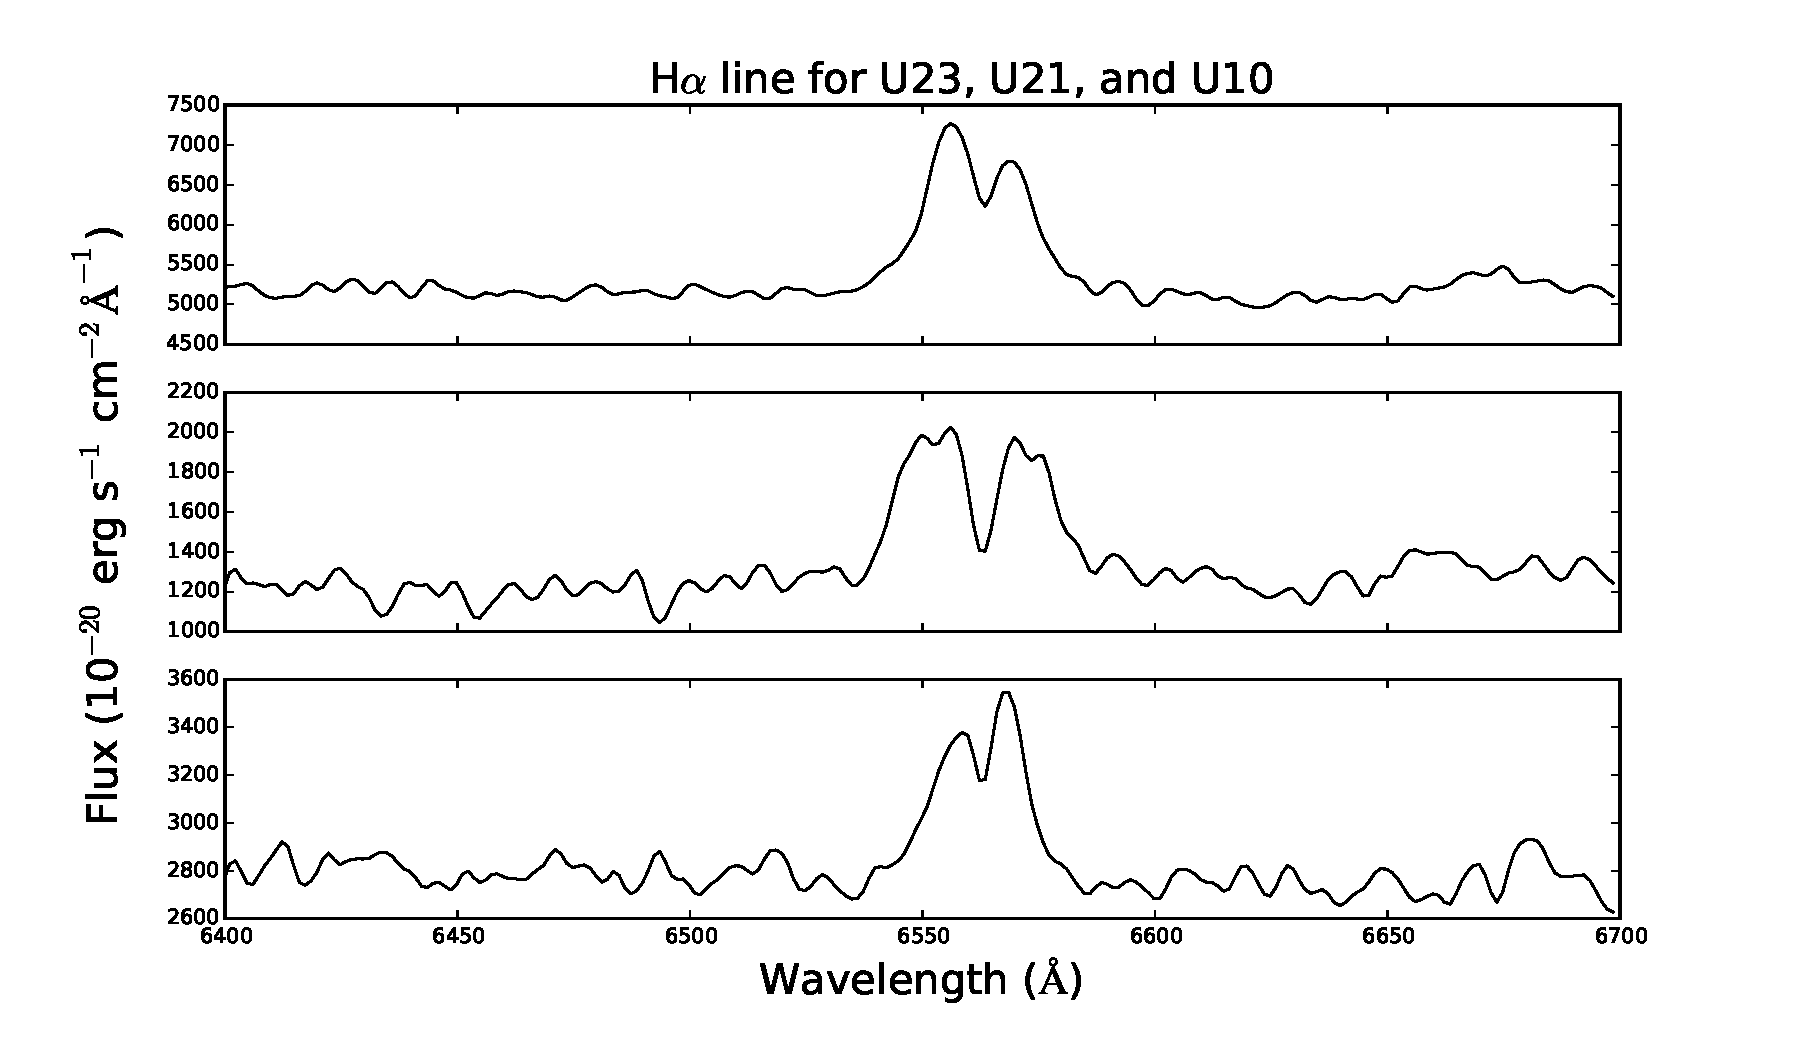
\includegraphics[scale=.5]{assets/images/todos.pdf}
\caption{Zoom of the spectra around H$\alpha$ for U23 (top), U21 (middle), and U10 (bottom)}
\label{fig:halphatodos}
\end{figure}

\begin{figure}[h]
        \centering
        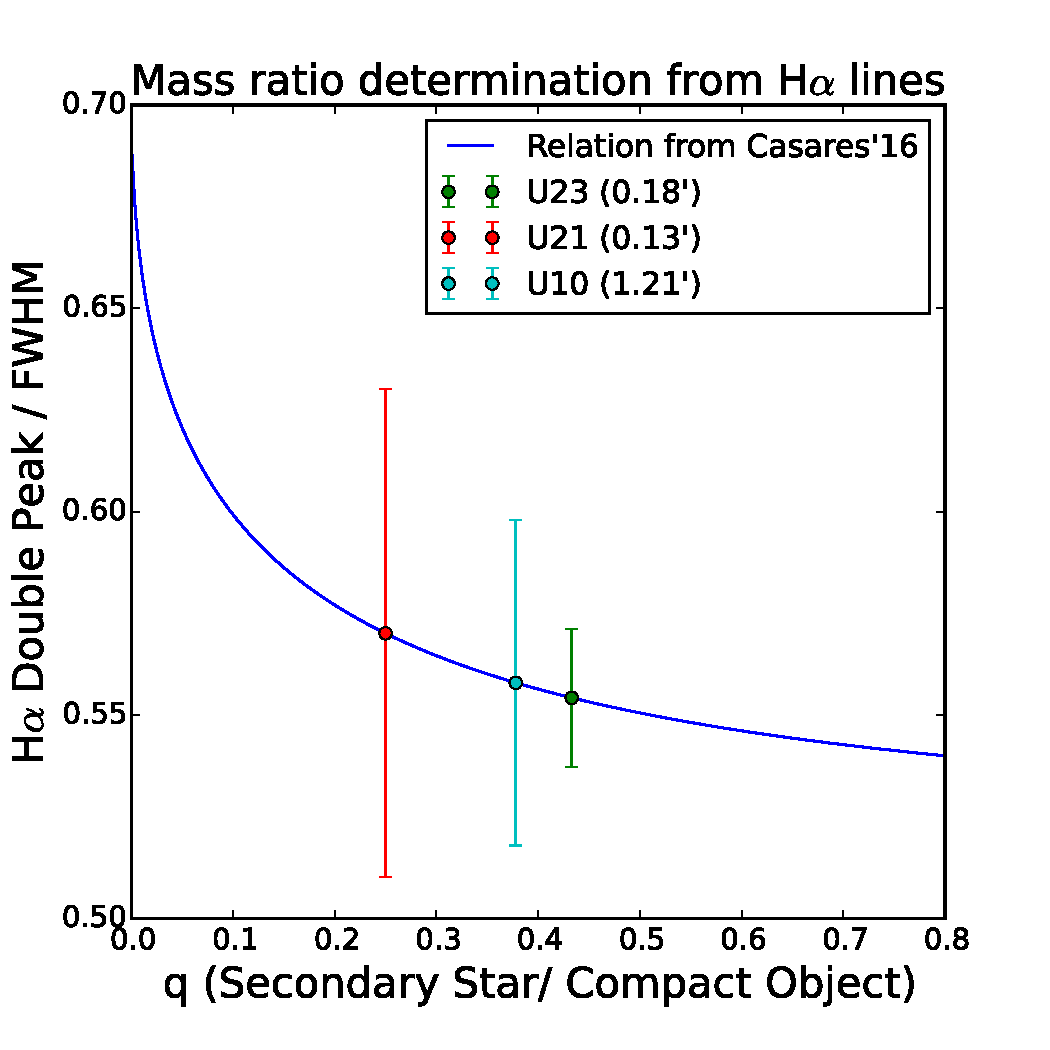
\includegraphics[scale=.5]{assets/images/mass.pdf}
\caption{Relation between the ratio of H$\alpha$ double peak separation to Full width at half maximum (FWHM) and the mass ratio (companion star over white dwarf mass) from \cite{casares_massration_20016}. The value in parenthesis is the projected distance to the cluster center. q for U23 is 0.433, for U21 is 0.25 and 0.3 for U10.}
\label{fig:mass}
\end{figure}

\subsection{Radial Velocity}

With the 8 different exposures of the center region and the strong H$\alpha$ line emission the radial velocity evolution of the CV can be trace. This is done by employing the cross-correlation algorithms of \cite{tonry_cross_1979}, as implemented in the IRAF Radial Velocity Analysis Package. This was done for U23, one of the brightest and one of the only two CVs in NGC 6397 for which the period have been measured \citep{kaluzny_time_2003}. The resulting radial velocity evolution is plotted in figure~\ref{fig:radU23}. The first exposure of 25 second for the first night was used as the template to calculate radial velocity shift. From the radial velocities measures we were unable to determine the period of the CV. This is due to the very large  errors bar. This suggest that longer integration time ($> 25$ seconds) is needed to be able to determine the period of the CVS in NGC 6397 with the MUSE instrument.   

\begin{figure}
        \centering
        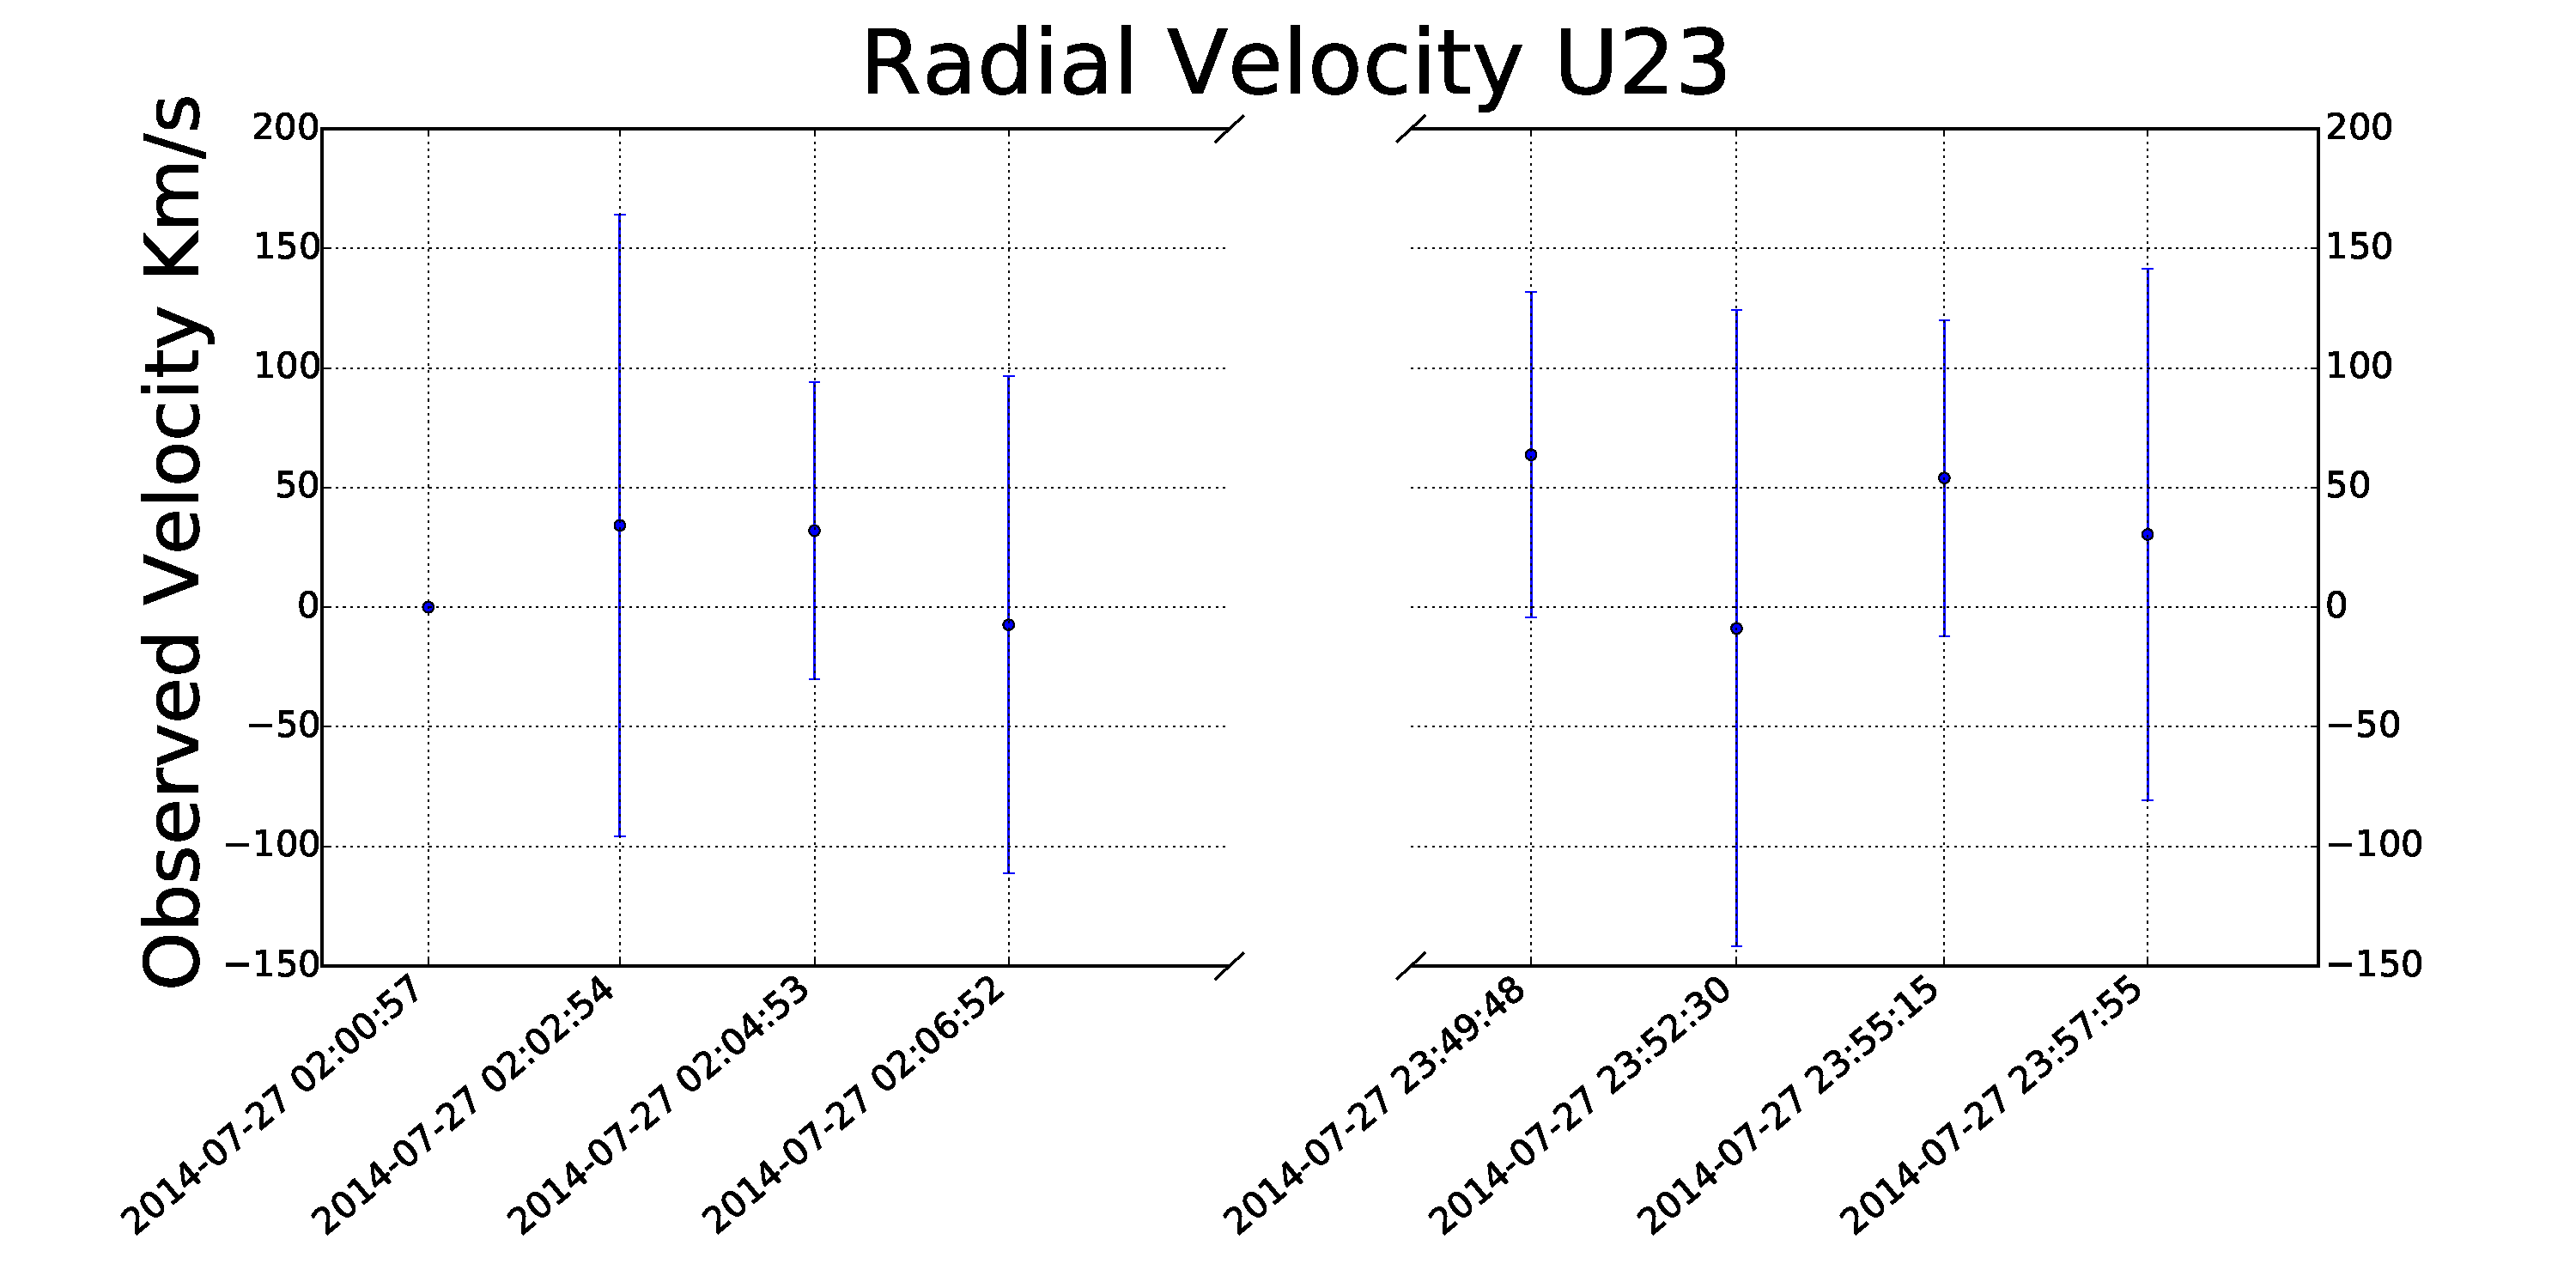
\includegraphics[scale=.3]{assets/images/radU23.pdf}
\caption{Radial velocity shift for U23. The radial velocity are measured using the first observing night as the reference template. With the available data we were unable to get a good estimate on the period of the CVs in NGC 6397, longer exposure time to obtained better quality spectra is needed.}
\label{fig:radU23}
\end{figure}

%\textbf{Note for Natalie: I am not sure what velocity from fxcor. Or the error. I The }

\section{Low-mass X-ray Binary}
Besides the population of CVs in NGC 6397 we also studied a LMXB located near the center in NGC 6397. Using of the available observation of the pointings at the center, we estimated the flux in the H $\alpha$ band to be $8.2 \times 10^{-18}$ erg/s/cm$^2$. This is a very faint object (R magnitude of $\sim 26$ \citep{heinke_improved_2014}). More integration time is needed to be able to get a spectra with a good signal-to-noise ratio and study the spectra of the LMXB. 


